\chapter{Machine Learning}

\section{The concept of machine learning}

For many decades computers have been an integral aspect of science, handling large amounts of data, completing tedious calculations and controlling experiments. For the most part the  machines were assigned discrete tasks. They step-wise followed commands previously designed by human users and had expected outcomes. 
For particle physics in particular, computers have been used to select and process interesting data from large samples. Making the processing of data possible at speeds beyond human capabilities. However the selection rules always had to be generated by the user, therefore requiring an in depth understanding of the underlying system. Machine learning presents a way for a program to establish its own decision rules, improving these over several iterations and thereby learning to solve the problem by itself.

There has been a great effort over the last decades trying to implement a way for machines to learn from known quantities and thereby enable them to analyse complex tasks ranging from voice recognition to object classification.
The efficiency and validity of a machine learning model is highly dependent on the human understanding of the problem at hand. The prerequisite to a successful model is the tuning of the degrees of freedom and parameters to the complexity of the assignment. This is called \emph{hyperparameter optimisation}. A task often proportional to the learning process itself.


Machine learning can be exemplified by drawing an analogy to human beings. In order to solve a problem, it must understand the system, evaluate a decision step and generate new decision steps.
Understanding a system means to be aware of all features and possibilities relevant to the task. Humans have their senses to easily break down their observations into useful features and concepts that can then be processed for decision making. A computer has no senses built in and for most tasks this means that the step of filtering information for a relevant subset of features has still to be done by humans or a good preprocessing algorithm.
Once a system has been converted to a subset of features usable by a computer, the step of making its own decisions has to be implemented. This can be done by weighting and interconnecting the information using structures inspired by neurons and synapses in the human brain. 


The structure and complexity of the network enables it to learn from data. In addition, a metric is introduced that measures the quality of the model, called the \emph{cost} or \emph{loss function}. This function allows the network to improve iteratively as a decrease in its value is considered an improvement by the network. Combined with an optimiser which suggests further steps, this function is a basis for a network to independently approach a good decision rule for a somewhat uninvestigated topic.

A very commonly used machine learning technique is the artificial neural network which on its own forms a broad field that builds the base of this work. The most important concepts of machine learning will be explained in the context of neural networks.

\section{Neural Networks}

The artificial neural network, or just neural network, is one of the most commonly known approaches to machine learning. Its structure is inspired by the neurons forming the human brain which is also where it gets its name from.\\
Instead of neurons a neural network consists of numerous very simple processors, called nodes. These nodes are usually structured into several layers. As presented in fig (todo). In addition to that there are several ways to structure and connect these nodes often times matching a certain problem. In this explanation only the most commonly way is explained. In that case each node of a layer is getting input from each node in the last layer and is outputting to each node of the following layer. Such a network structure is shown in figure \ref{fig:nodes_nomenclature}. It describes the step between a node and the previous layer. The underlying math will be explained in detail later. This is called a feed-forward neural network.

\begin{figure}
	\centering
	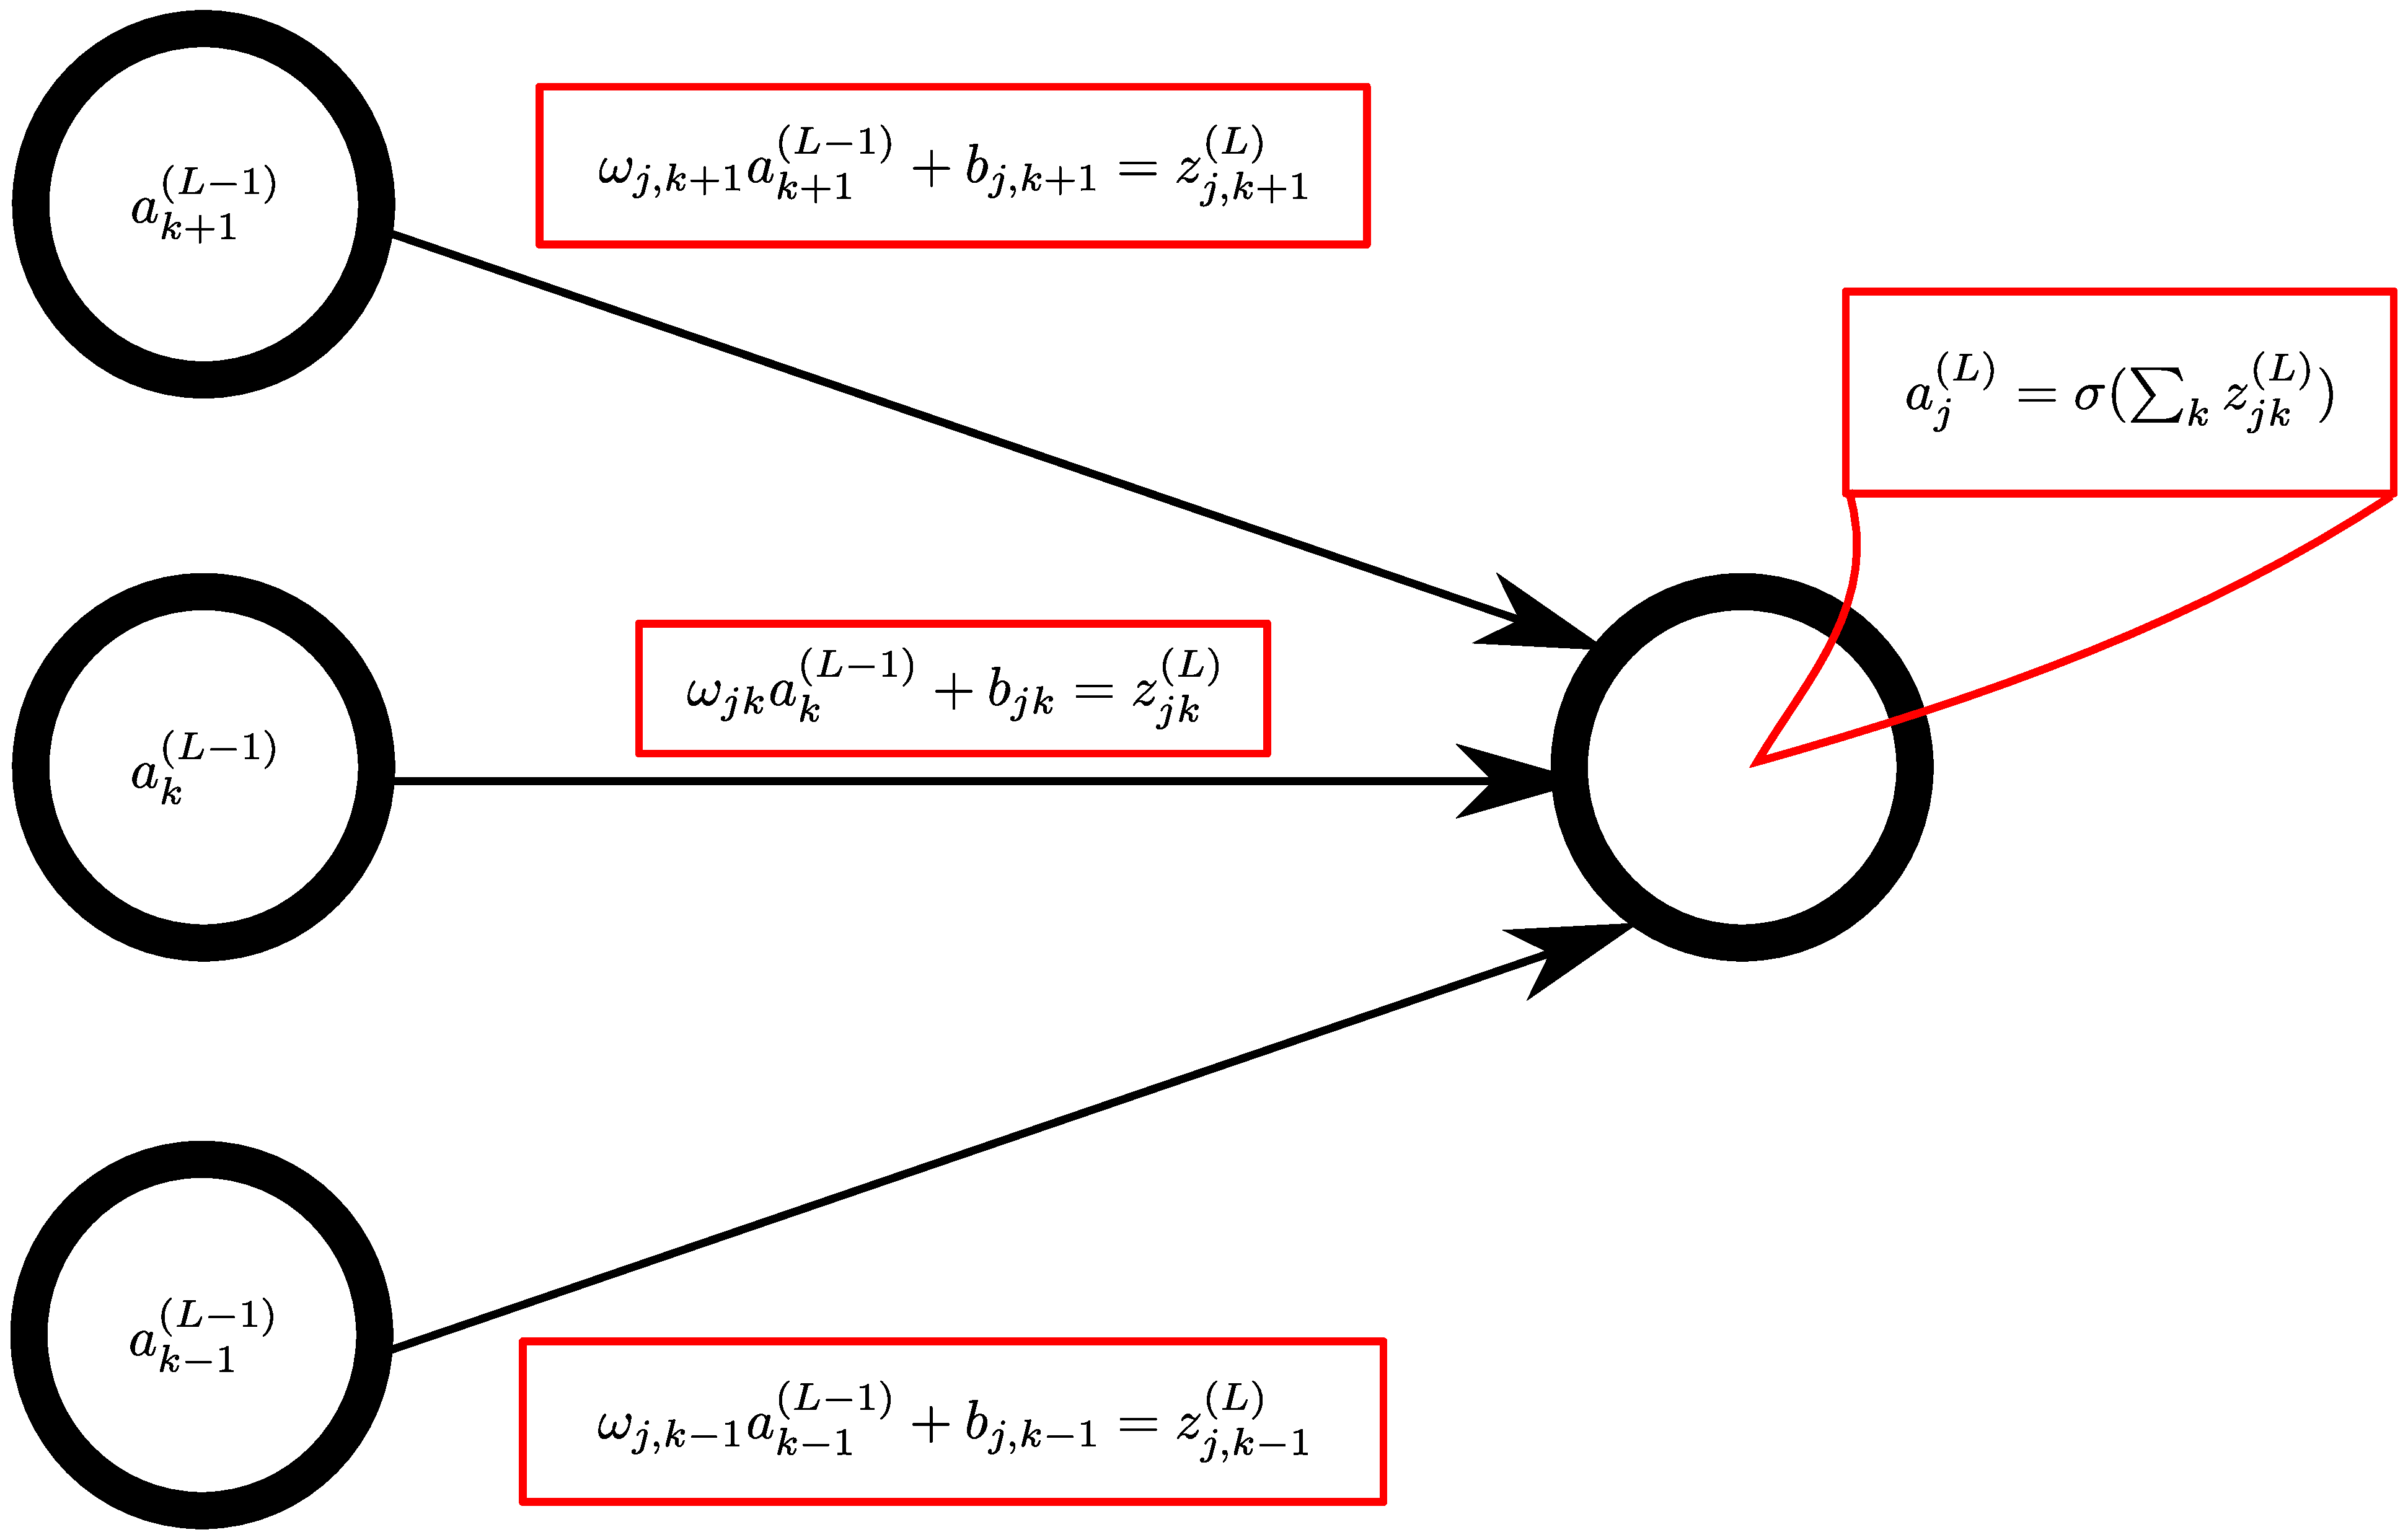
\includegraphics[scale=0.18]{figures_ML/nodes_nomenclature.eps}
	\caption{Network propagation from layer $(L-1)$ to layer $L$}
	\label{fig:nodes_nomenclature}
\end{figure}


\subsubsection{The input layer}

To understand a task and draw reasonable conclusions first the underlying system has to be understood. Its features need to be found and summarised. The human brain is capable of investigating unknown systems and learn the features that are the most unique or interesting. For that it has its senses to explore the system and process them later. To allow a machine to do something similar the unknown system has to be represented in a way that it is clear for the network what to look out for. This is usually the task that needs the most preprocessing by the user. The simplest case is to submit a list of variables to the network. In particle physics this could be kinematic variables of the particles in an event.
The input to a neural network is just given to the input layer of nodes and then processed through each following layer. For different tasks different layers might deal with different parts of the information but in this work the linear way of giving all information used to an input layer and then processing it is used.

\subsubsection{Decision making process}

Computers being not much more than very powerful calculators, excel at performing high numbers of clearly defined calculations. The trick is that the task has to be defined clearly. There usually is no fuzziness.\\
This is very different for the human brain. We rely on a certain fuzziness when processing information through a net of neurons where the output of every neuron is taken as input for the surrounding neurons. The challenge of machine learning is to represent this fuzziness by many somewhat discrete calculations. In the neural network the neurons and their fuzzy interaction is represented by the nodes which are very simple processors. Like neurons each node can use input from many other nodes to create a new output signal. Thereby the input information can be linked to each other in numerous ways. Combined with a weighting system this allows to create complex models and match a variety of problems.

The input of every node is the weighted output of all previous nodes as shown in equation \eqref{eq:node_input}. $z_j^L$ is the input to the $j$-th node in the $L$-th layer. $\omega_{jk}^L$ is the weight from the $k$-th node in the previous layer to this node, $a_k^{L-1}$ is that node's output and $b_k$ the relevant bias. The sum indicates that all $k$ previous nodes contribute to the input to the $j$-th node.

\begin{align}
    z_j^L = \sum_{k=0}^{N} \omega_{jk}^L a_k^{L-1} + b_k
    \label{eq:node_input}
\end{align}
The weight allows to predict which variables are linked to each other or allow for better decision rules when combined but also easily to weight the importance of features. Furthermore the output of each node is non binary allowing to combine the input signals to a single output. This is called the activation function of a node. A common choice is the sigmoid function as presented in equation \eqref{eq:sigmoid_activation}.~\cite{chollet2015keras}

\begin{align}
    a_j^L = \sigma ( z_j^L ) = \frac{1}{1 + e^{z_j^L}}
    \label{eq:sigmoid_activation}
\end{align}

The sigmoid function has output between $0$ and $1$ which is often times what one wants for nodes especially for the final layer as we are looking for predictions of outcome probabilities. A selection of further activation functions is shown in table \ref{tab:activation_functions}.

\begin{table}[]
\centering
\begin{tabular}{l|l|l}

Name                    & Function & Plot \\ \hline
Sigmoid                 &$f(x) = \frac{1}{1 + e ^{-x}}$        &   \raisebox{-0.5\height}{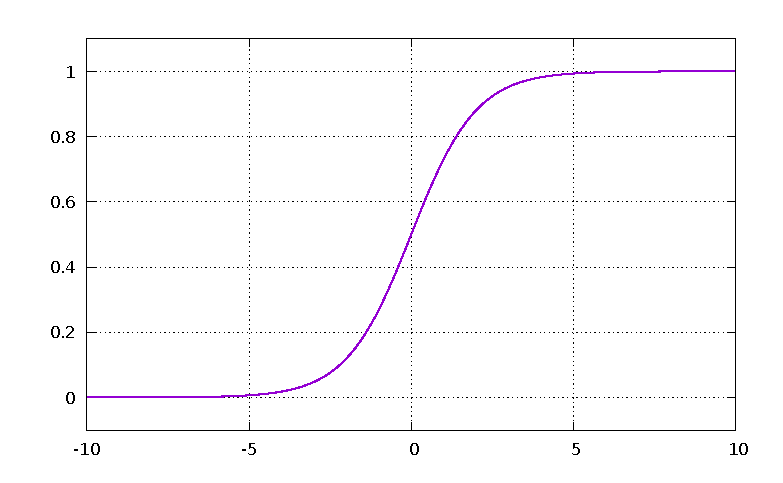
\includegraphics[scale=0.3]{figures_ML/sigmoid}}              \\ \hline
Tangens Hyperbolicus    &$f(x) = \frac{2}{1 + e ^{-2x}} -1$        &        \raisebox{-0.5\height}{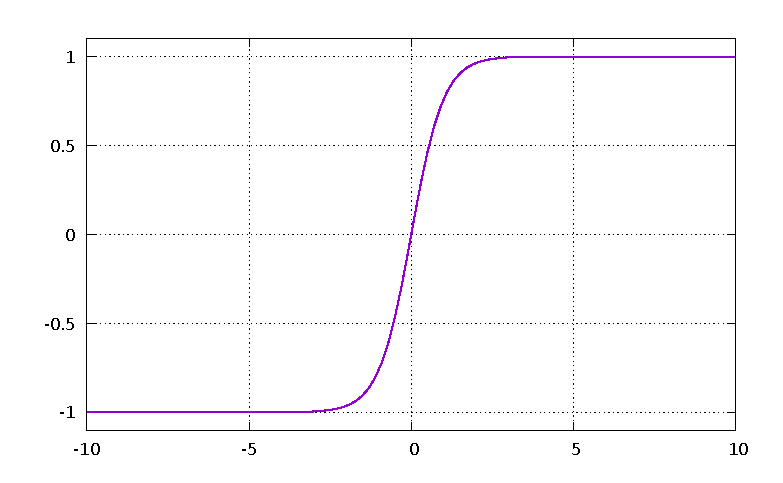
\includegraphics[scale=0.3]{figures_ML/tanh}}         \\ \hline
Rectified Linear Unit, \textsc{ReLu}   &$f(x) =
  \begin{cases}
    0       & \quad \text{if } x < 0\\
    x  & \quad \text{if } x \geq 0
  \end{cases}$     &      \raisebox{-0.5\height}{ 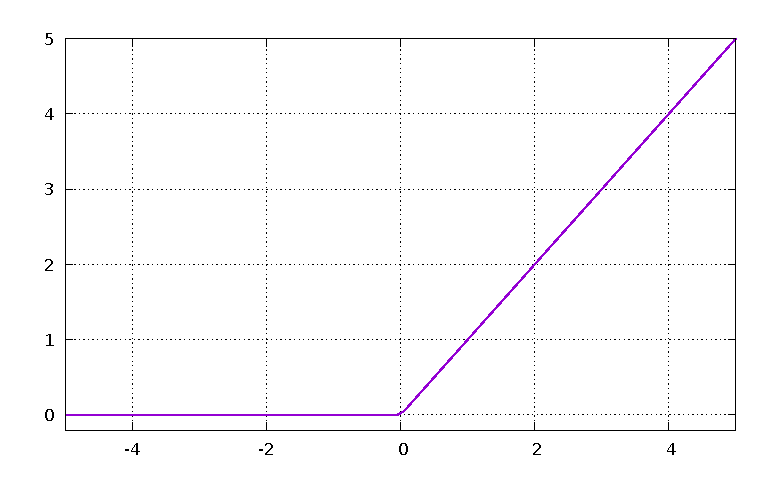
\includegraphics[scale=0.3]{figures_ML/relu}}          \\ \hline
Exponential Linear Unit, \textsc{ELU} &$f(x) =
  \begin{cases}
    \alpha ( e^x -1 )     & \quad \text{if } x < 0\\
    x  & \quad \text{if } x \geq 0
  \end{cases}$      &        \raisebox{-0.5\height}{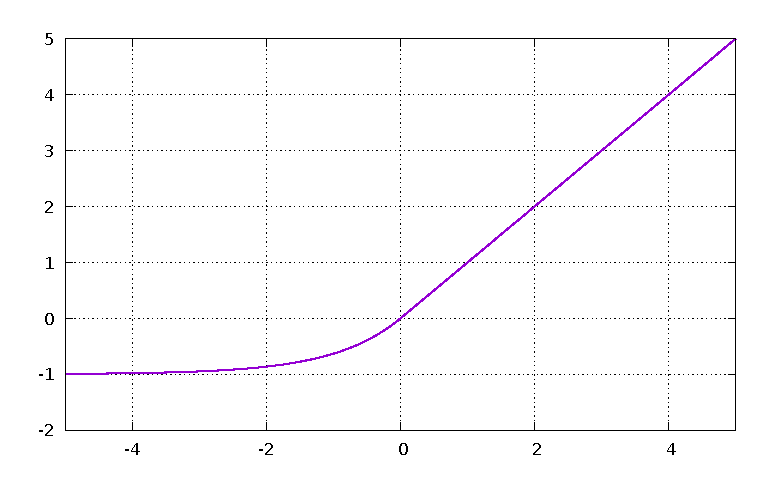
\includegraphics[scale=0.3]{figures_ML/elu}}         \\ 
\end{tabular}
\caption{Selection of activation functions taken from the Keras documentation. \cite{chollet2015keras}}
\label{tab:activation_functions}
\end{table}

For this thesis especially the exponential linear unit or \textit{elu} and the rectified linear unit or \textit{relu} were tested.
\textit{Elu} is good for converging the cost to zero rather fast and has the possibility of negative output.
\textit{relu} allows for the same benefit as sigmoid while requiring less computational power for the simply linear output for positive values.

Of course the network does still not know the task assigned to it but if we add a cost function to estimate the quality of a decision rule created by a certain combination of the input we can easily make the network approach a better decision rule and hopefully the solution of the problem as the cost function just needs to be minimised. In this work the cost function will be called the loss of the model.

In supervised learning the network is trained with a set of known data. Each event of the training set has a label representing the true outcome value referred to as just label or truth label. Comparing this truth information to the network output makes it very easy to calculate the loss as the deviation of the network output from the desired truth output. A possible loss function is the crossentropy or just binary crossentropy for a binary output result. As in this work the result is binary, signal and background, the binary crossentropy is the natural choice. Equation \eqref{eq:binary_crossentropy} shows the underlying function where $p$ is the estimated probability for the outcome $\hat{y}$ and $y$ is the label for a  correct or incorrect guess.

\begin{align}
    C = -(y \log p + (1 - y) \log (1 - p) )
    \label{eq:binary_crossentropy}
\end{align}

The loss is the foremost observable for the training quality. This quality must not be mixed up with the overall quality of the model as for the loss only the data trained on is taken into account but not a test data set.

\subsubsection{Optimizers - Choosing the next step}

The probability interaction of the nodes combined with the loss function enables a network not only to create a model but also to evaluate it. The last missing part is an algorithm that can estimate a step to a model that further minimises the loss. One could certainly do this randomly until the network finds a very low costed decision rule if infinite computational power were provided but that would neither be an efficient nor the desired learning process.

The output of each node in the final layer is defined by the weighted and biased information of the previous nodes and lastly the activation function. For one connection therefore there are three variables that have impact on the loss. Summarising this information for all nodes in a vector defines the loss-vector. The gradient of this vector is an estimator for the impact of each parameter on the overall loss and thereby gives a prefered direction for the model. Updating a network's parameters based on this gradient is called backpropagation. The algorithm works as follows:

\begin{enumerate}
    \item A certain set of input variables is iterated through all layers of a network resulting in an estimator $\hat{y}$ at each output node.
    \item The sum of deviations from the true value at all output nodes is determined as the loss $C$ of the setup. The loss just defines how good the model is.
    \item The gradient of the loss is calculated as the partial derivative of all network parameters
    \begin{align*}
        \frac{\partial C}{\partial a_k^{L-1}} = \sum_{j=1}^N \frac{\partial z_j^L}{\partial a_k^{L-1}} \frac{\partial a_j^L}{\partial z_j^L}\frac{\partial C}{\partial a_j^L}
    \end{align*}
    \item The parameters are then updated backwards through the layers following the negative loss gradient.
\end{enumerate}

This backpropagation algorithm is the backbone of the neural network's learning process.

The decision step based on the gradient defined above is specified by the networks optimizer and deserves a bit more attention. There is different choices of optimisers trying to accommodate different problems as well as some parameters important to understand and tune for an effective training. The length of a learning step has to match the problem's topology to properly let the model converge. First we define the gradient $g$ in a more general way. The batch size is $m$, $f$ is the network for configuration $\theta$ and output $\hat{y}$. The target is $y$.

\begin{align}
    g = \frac{1}{m} \nabla_{\theta} \sum_j L(f(\hat{y}^j; \theta), y^i)
\end{align}

The configuration $\theta$ is then updated using the gradient and a constant $\eta$ called the learning rate as it determines the step size for each update.

\begin{align}
    \theta \prime = \theta - \eta g
\end{align}

Optimisation processes like this are gradient descent based optimisers and can be considered the basis of all optimisers. Depending on the choice they might be based on the whole training sample or just a mini batch of the sample. The most basic form has the learning rate as its only hyperparameter. A good learning rate should be small enough to avoid oscillations but high enough to approach a minimum efficiently fast. A good estimate is given by the Robbins Monro condition:

\begin{align}
    \sum_k \eta_k = \infty\\
    \sum_k \eta_k^2 < \infty
\end{align}

As the choice of learning rate will not be perfect for every part of the problem's topology, momentum $\nu$ can be introduced as a second parameter to the optimizer.~\cite{chollet2015keras} The effect desired is that the stepsize becomes greater when the slope is long and the minimum is still far away and to be shorter when approaching the minimum. Momentum scales each step by how aligned previous steps were. That means it will allow avoiding local minima or moving slowly along a slope by enlarging steps at the beginning of the training but also will slow down at the end of the training when the steps become shorter. It promises to speed up the training with less risk of large oscillations which a large learning rate would probably result in. Momentum also takes a single scaling hyperparamter $\alpha$ and is updated each step following: 

\begin{align}
    \nu^{\prime} = \alpha \nu - \eta \frac{1}{m} \nabla_{\theta} \sum_j L(f(\hat{y}^j; \theta), y^j)\\
    \theta^{\prime} = \theta + \nu^{\prime}
\end{align}

Alternatively one can use Nesterov momentum~\cite{chollet2015keras} which is a more advanced adoption of momentum and updates the step a further time after applying the gradient: 

\begin{align}
    \nu^{\prime} = \alpha \nu - \eta \frac{1}{m} \nabla_{\theta} \sum_j L(f(\hat{y}^j; \theta + \alpha \times \nu), y^j)\\
    \theta^{\prime} = \theta + \nu^{\prime}
\end{align}

Lastly it can be helpful to decrease the learning rate of the network stepwise while approaching a minimum to avoid oscillations or leaving the minimum in general further. This can be accomplished by the hyperparameter of learning rate decay. It just decreases the learning rate in each iteration $t$ by a small hyperparamter $\phi$ following the assumption that smaller steps are sufficient close to the minimum.~\cite{chollet2015keras}

\begin{align}
    \eta^{\prime} = \frac{\eta}{1 + \phi t}
\end{align}

\subsubsection{Adaptive optimisers}

In addition to the purely gradient based optimisers there are adaptive optimisers. Learning rate and momentum as previously described are difficult to tune to every part of the training process as the topology of the problem might rapidly change. Therefore adaptive optimisers update their parameters based on the training process. There is a set of adaptive optimisers.~\cite{chollet2015keras}\\
Often the adaptive optimiser of choice is \textsc{Adam}.~\cite{2014arXiv1412.6980K} \textsc{Adam} updates both, its learning rate and its momentum over the course of the training based on an exponentially decaying average of past gradients and past, squared gradients. The average makes sure that the parameters keep getting updated based on past steps. They should be decaying as otherwise the parameters would rapidly shrink. The decay of the averages is defined by a hyperparameter $\beta$.

\begin{align}
    \hat{g}^2 = \frac{\sum g^2}{1 - \beta_1^t}
\end{align}

\begin{align}
    \hat{g} = \frac{\sum g}{1 - \beta_2^t}
\end{align}

The model's parameters are then updated according to:

\begin{align}
    \theta^{\prime} = \theta + \frac{\eta}{\sqrt{\hat{g}^2} + \epsilon} \hat{g}
\end{align}

\textsc{Adam} is often considered a very good algorithm as it contains many corrections to hyperparamters during the training and thereby allows for easier optimisation but it also needs more computational power.


\section{Regularisation and Optimisation}

Fluctuations and noise in the training sample can be a big problem for a model trained on the sample as a neural network might pick noise and random fluctuations up as features for the decision rule.\\
This basically is the process of overfitting. The network sees way more features to work with than those actually present in reality or even in a different test sample. The most extreme scenario is that your network is large and deep enough to pick up every single feature in the training sample. If that happens the training error becomes very low and indicates a very good decision rule. For a different sample this decision rule is at most very unreliable but probably strictly wrong resulting in a high test sample error. The network just picked up and remembered every single feature in the training sample instead of general correlations. It becomes a mask of the sample.\\
A possible way to solve this issue is to stop the training early or to find a good way when to stop the training. This way noisy features might not yet have been picked up by the training. Then again this might also lead to a suboptimal result of the overall training as one cannot be sure that the correct features always get picked up first. Especially when large systematic uncertainties have to be dealt with.\\
More sophisticated approaches are called regularisations of a neural network. The most commonly used solution is a so called Dropout layer described in the subsection \ref{sec:dropout}. Additionally a batch normalisation can have an effect of regularisation and is therefor introduced in this section as well.

\subsection{Dropout}
\label{sec:dropout}

Dropout is attempting to keep the network from relying on subdominant features too much by removing different nodes in each iteration. This forces the network to build models that are not based on strong correlations between nodes. The weights become less interdependent. To simplify it a lot it means training several neural networks depending on which nodes are turned on during a training epoch. It keeps the training in motion for a large number of epochs.\\
Dropout is added to each layer of a network and can also be  restricted to a subset of layers too. It slows down the training as the additional motion slows down the process of finding a minimum but it also accelerates each epoch slightly as it simplifies the network architecture. 

\begin{figure}
	\centering
	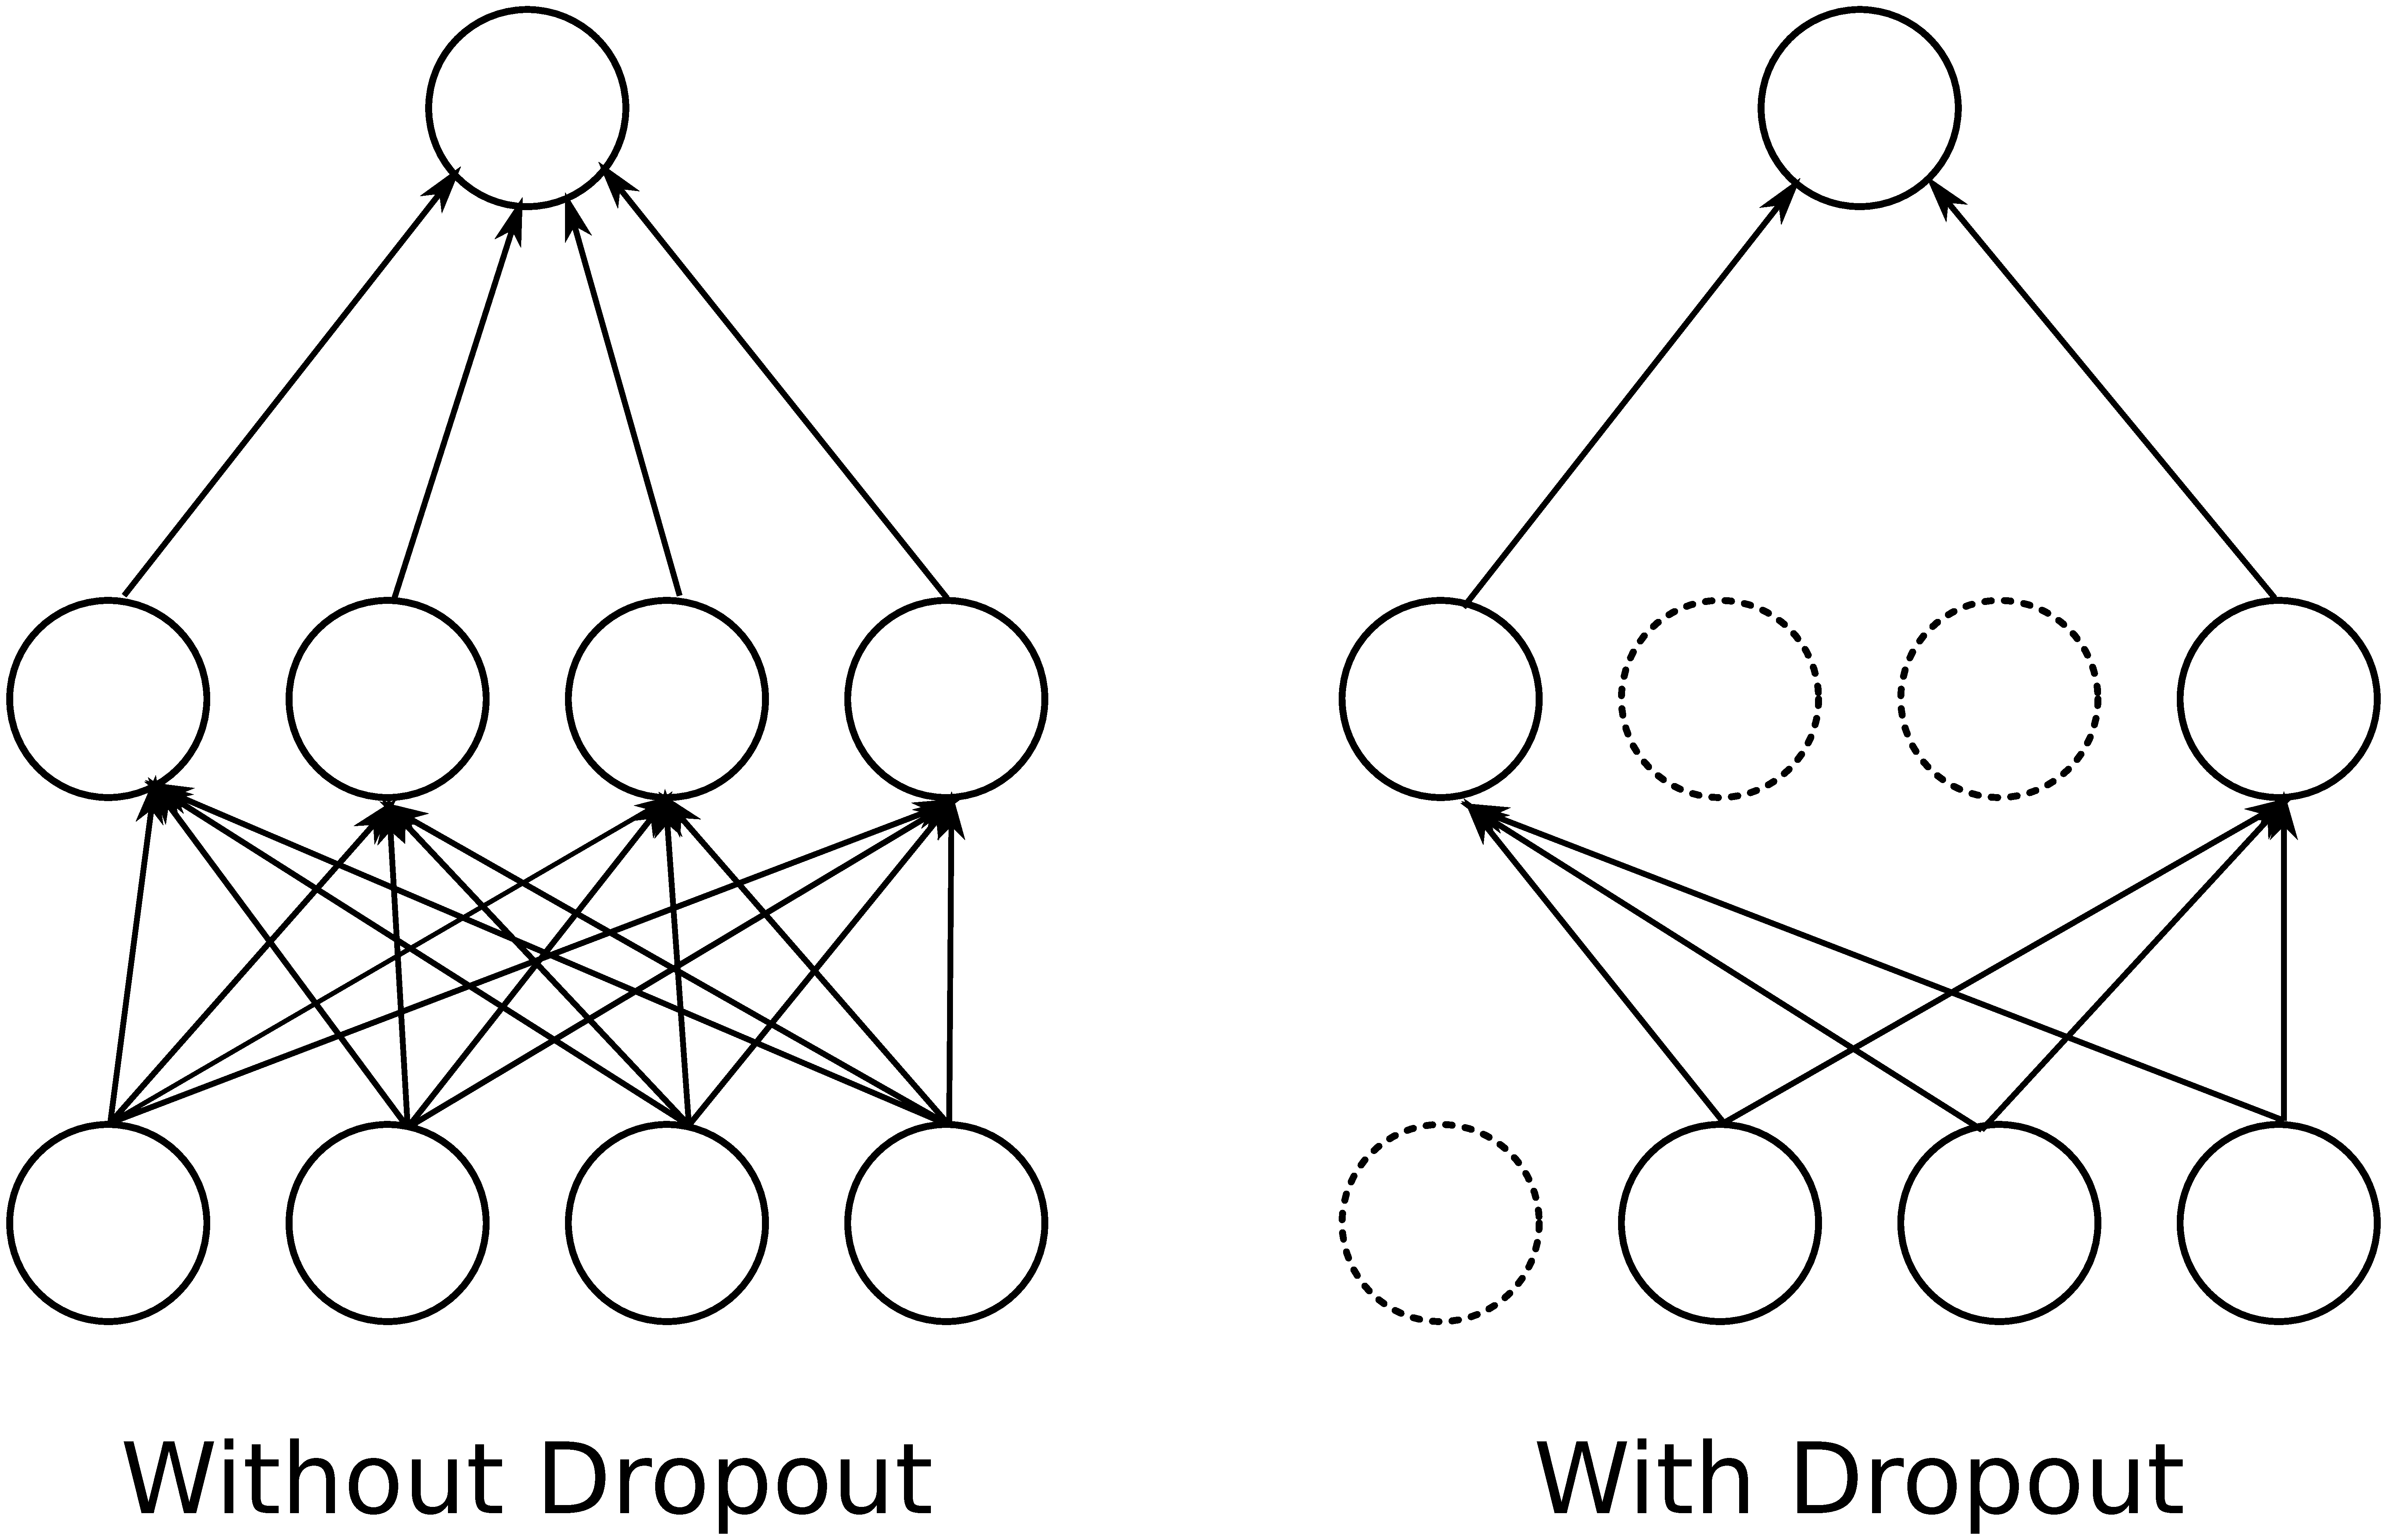
\includegraphics[scale = 0.1]{figures_ML/dropout.eps}
	\caption{Sketch of network before and after the inclusion of dropout. On the left hand side dropout is not applied and all nodes are connected. On the right hand side the dashed circles are nodes excluded by dropout and therefor not connected to the other nodes.}
	\label{fig:dropout}
\end{figure}



\subsection{Batch normalization}
\label{sec:batch_norm}

In supervised learning the training result is heavily dependent on the set of data the network is trained on. This means that the performance might change a lot when the test data is very different. Imagine a classifier distinguishing between pictures that show cars and pictures that do not show cars. If the training set contains predominantly green cars the colour green might end up as a strong indicator for  the classification car. In general the colour green will not be as dominant and the network will perform slightly worse when trying to classify cars of a different colour. Formally such a change of input is called a covariance shift.\\
A way to reduce the effect of covariance shift is batch normalization. The output of nodes in general and the weight of a connection in a neural network is not necessarily limited allowing for certain connections to be really dominant and overshadowing less dominant features. We want to avoid this as the dominance of some features might just be present in the training sample. This can be achieved by normalizing the output of each layer in the network to the total output and thereby minimising the effects of strongly overrepresented features. This is done by normalizing each output to the mini-batch mean $\mu_B$ and the mini-batch standard deviation $\sigma_B^2$.

\begin{align}
    \mu_B = \frac{1}{m} \sum_i x_i\\
    \sigma_B^2 = \frac{1}{m} \sum_i (x_i - \mu_B)^2\\
    x_{i,norm} = \frac{x_i - \mu_B}{\sqrt{\sigma_B^2 + \epsilon}}
\end{align}





\section{Adversarial Neural Networks}

This main part of this work is the examination and training of an adversarial neural metwork. An adversarial neural network consists of a classifier and a second network that tries to regularise the output of the first classifying network.\\
In this section the concept of an adversarial neural network is motivated and the underlying mathematics as originally stated in paper~\cite{2014arXiv1406.2661G} are presented.

\subsection{The adversarial neural network}

Neural networks have been very efficient for classifying tasks but less successful for generative tasks. This was the original problem that gave birth to the idea of a generative adversarial network. Generative networks often times have output that is very easy to distinguish from real samples. The solution suggested is adding a classifier that tries to distinguish between generated samples and real samples. As long this adversary is able to accomplish this task the first network fails at its generative task. Training the two networks against each other should disincentive the generative network from using the features not dominant in real samples.\\
In this work the first network is not a generator but a classifier separating signal events from background events in a Monte Carlo simulation. These simulations contain systematic uncertainties. The classifier should not be too dependent on variables with high systematic uncertainties. If the classifier has these strong dependencies on systematic uncertainties it might lead to a high co-variance shift. Instead of a generated sample and a truth sample a so called nominal sample and systematic samples are used as input for the second network. Systematic samples have slightly different distributions than the original samples because of changes to the variables with the systematic uncertainties. Training the second network on determining whether it is looking at a nominal or a systematic sample allows to estimate how dependent the model is on variables with high systematic uncertainties. Training the classifier against the adversarial network promises to reduce the effect of systematic uncertainties on the model.
Mathematically this comes down to a minimax decision rule or a competition between two neural networks. Let us call the classifier $Net1$ and the adversary $Net2$ then the problem becomes:

\begin{align}
    \min_{Net1} \max_{Net2} V(Net1, Net2) = \mathbb{E}_{\mathit{x} \sim \rho_{data}} [ log Net1(\mathit{x}) ] + \mathbb{E}_{\mathit{z} \sim \rho_{sys}} [ log (1 - Net2(\mathit{z}) ) ]
\end{align}

$V(Net1, Net2)$ is the combined value function for the two adversary networks. The first network is trained to be an optimal classifier represented by $log Net1(\mathit{x})$ while the second network is trained to distinguish between the nominal and systematics distribution $\mathit{z} \sim \rho_{sys}$ represented by $log (1 - Net2(\mathit{z}))$. In theory the first classifier should be trained slowly and kept close to its optimum while the second network slowly learns and allows the first network to adapt to it. This is achieved by training the two networks successively over multiple iterations using a combined value function.
As this value function a combined loss function is used. It is just the difference between the two separate loss functions with a hyperparameter $\lambda$ to control the impact of the adversary as shown in equation \eqref{eq:adversarial_loss}.

\begin{align}
    \mathcal{L} = L_{net1} - \lambda L_{net2}
    \label{eq:adversarial_loss}
\end{align}

In the first step of each iteration the first network is trained using the combined loss function $\mathcal{L}$. In the second step the second network is trained using its simple loss function $\lambda L_{net2}$. Each of the networks has the usual set of hyperparameters to optimise explained in detail in the previous sections missing.


